\chapter{Testy urządzenia}
\section{Analiza poboru prądu układu}
\begin{figure}[h]
    \centering
    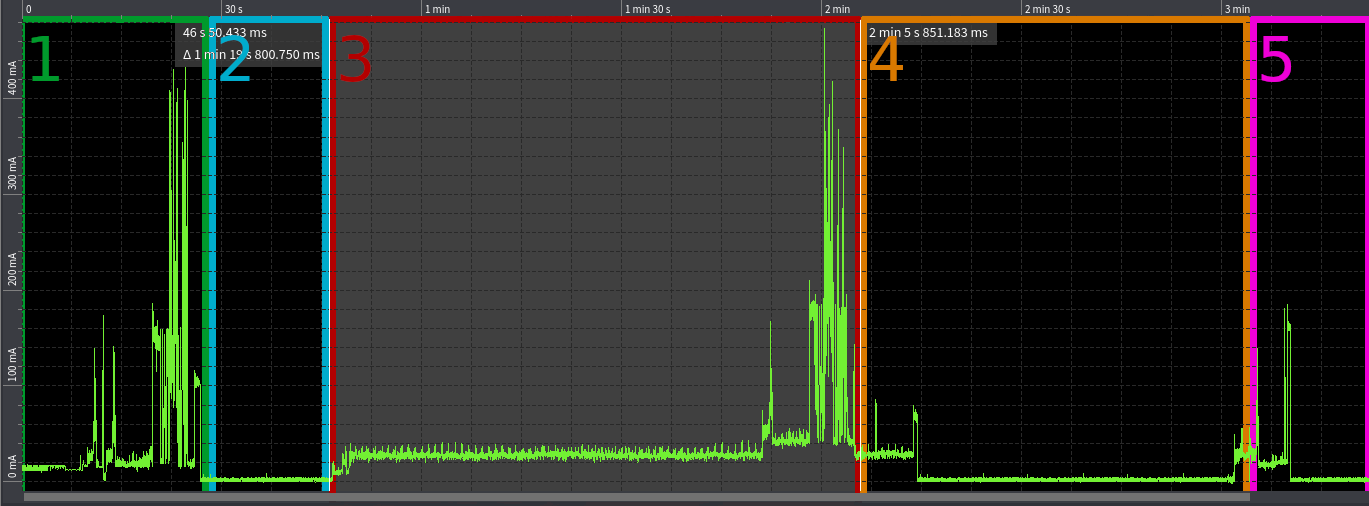
\includegraphics[width=16cm]{Graphics/connection_with_fix_divided.png}
    \caption{1. inicjalizacja urządzenia. 2.Tryb uśpienia. 3. Wyzwolenie alarmu oraz wysłanie lokalizacji. 4.Oczekiwanie wysłanie kolejnego powiadomienia. Buzzer włączony. 5.Przerwanie alarmu przyciskiem, uśpienie układu.}
    \label{img:current_summary}
\end{figure}